\documentclass{beamer}
\usetheme{Warsaw}

\setbeamercolor{normal text}{fg=white,bg=black!90}
\setbeamercolor{structure}{fg=white}

\setbeamercolor{alerted text}{fg=red!85!black}

\setbeamercolor{item projected}{use=item,fg=black,bg=item.fg!35}

\setbeamercolor*{palette primary}{use=structure,fg=structure.fg}
\setbeamercolor*{palette secondary}{use=structure,fg=structure.fg!95!black}
\setbeamercolor*{palette tertiary}{use=structure,fg=structure.fg!90!black}
\setbeamercolor*{palette quaternary}{use=structure,fg=structure.fg!95!black,bg=black!80}

\setbeamercolor*{framesubtitle}{fg=white}

\setbeamertemplate{navigation symbols}{}%remove navigation symbols

\setbeamercolor*{block title}{parent=structure,bg=black!60}
\setbeamercolor*{block body}{fg=black,bg=black!10}
\setbeamercolor*{block title alerted}{parent=alerted text,bg=black!15}
\setbeamercolor*{block title example}{parent=example text,bg=black!15}

\DeclareMathOperator*{\mymax}{max}
\DeclareMathOperator*{\argmax}{arg\,max}
\DeclareMathOperator*{\argmin}{arg\,min}
\DeclareMathOperator*{\ForAll}{\bigwedge}
\DeclareMathOperator*{\Exists}{\bigvee}
\newcommand{\hoch}[1]{^{#1}}

\AtBeginSection{\frame{\usebeamerfont{section title}\insertsection}}

\newcommand\etal{et.\,al.}

\usepackage[english]{babel}
% avant, courier, chancery, times, palatino, bookman, 
% newcent, utopia, charter
%\usepackage{times}

\usepackage{natbib}
\usepackage{booktabs}
\usepackage{tabularx}

\usepackage[latin1]{inputenc}
\usepackage[T1]{fontenc}
\usepackage{multicol}
\usepackage{mdwtab}
\usepackage{booktabs}
\usepackage{tabularx}
\usepackage{txfonts,textcomp}
\usepackage{amsmath}
\usepackage{amsfonts}

\setlength\parindent{0cm}
\setlength\parskip{2mm}
\setbeamerfont{gross}{size=\large}
\setbeamerfont{quetsch}{size=\tiny}
\setbeamerfont{klein}{size=\footnotesize}
\newcommand\w[1]{\mathbf{#1}}

% example list spacing
\newcommand\ml{\setlength\itemindent{-11mm}}

	\title{Structured Prediction and PyStruct} 
    \author{Andreas M\"uller}%

	\begin{document}

	\begin{frame}[plain]
		\titlepage
	\end{frame}


    \section{Motivation}
    % output space combinatorial
    % output space depends on input space
    % model correlations
    \begin{frame}
        \frametitle{Multi-Label Classification}

        \begin{table}
            \begin{tabularx}{\linewidth}{lccccc}
                \toprule
                & \footnotesize{Politics} & \footnotesize{Sports} & \footnotesize{Finance} & \footnotesize{Domestic} & \footnotesize{Religion}\\
                \cmidrule{2-6}
                News Story1 & 1 & 0 & 0 & 1 & 1\\
                News Story2 & 0 & 1 & 0 & 1 & 0\\
                News Story3 & 0 & 0 & 1 & 0 & 0\\
                \bottomrule
            \end{tabularx}
        \end{table}

        \begin{visibleenv}<2>
        \begin{table}
            \begin{tabularx}{\linewidth}{lccccc}
                \toprule
                & \footnotesize{Owns Car} & \footnotesize{Smokes} & \footnotesize{Married} & \footnotesize{Self-Employed} & \footnotesize{Has Kids}\\
                \cmidrule{2-6}
                Customer1 & 1 & 0 & 1 & 0 & 1\\
                Customer2 & 1 & 1 & 0 & 1 & 0\\
                Customer3 & 0 & 1 & 1 & 0 & 0\\
                \bottomrule
            \end{tabularx}
        \end{table}
        \end{visibleenv}
        
    \end{frame}

    \begin{frame}
        \frametitle{Sequence Tagging}
        \begin{columns}[t]
            \column{.2\linewidth}
            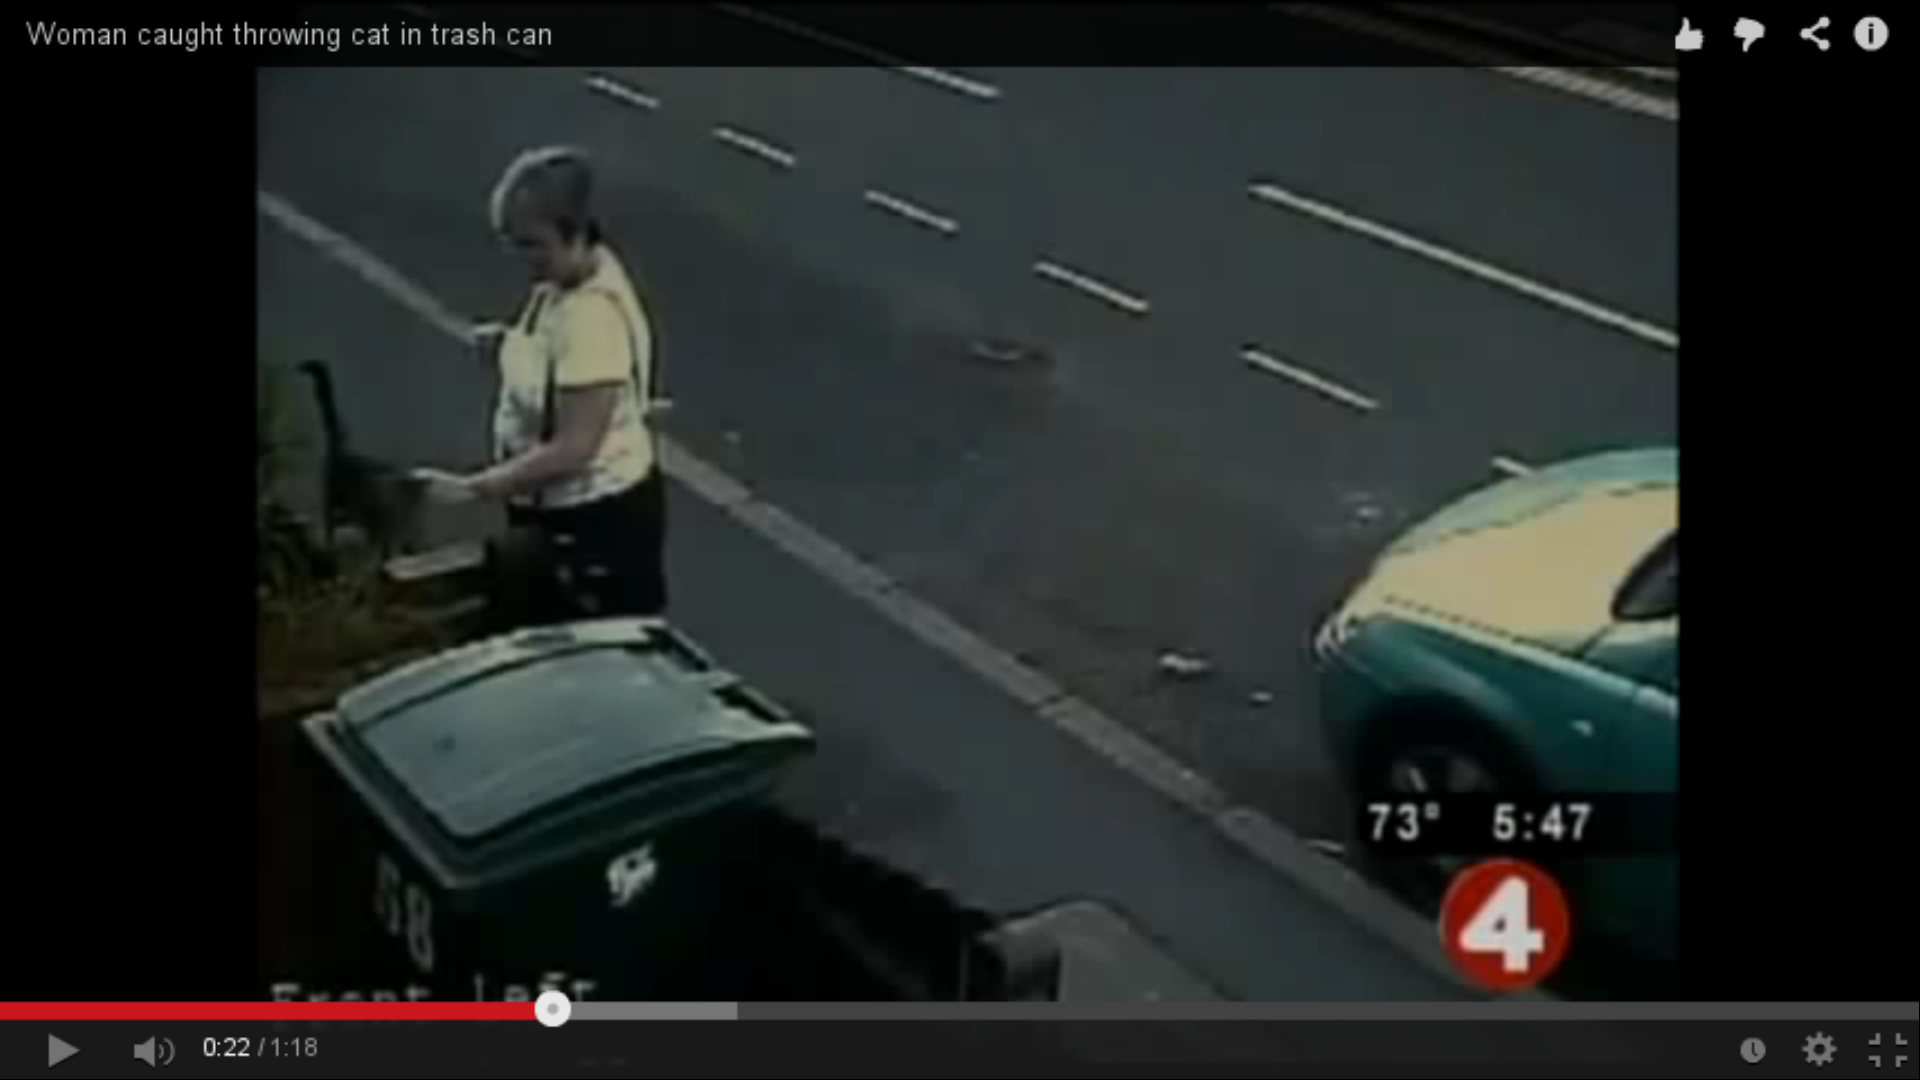
\includegraphics[width=\linewidth]{images/stroke1}\\
            \begin{visibleenv}<2->
                \tiny{Stroke cat.}
            \end{visibleenv}

            \column{.2\linewidth}
            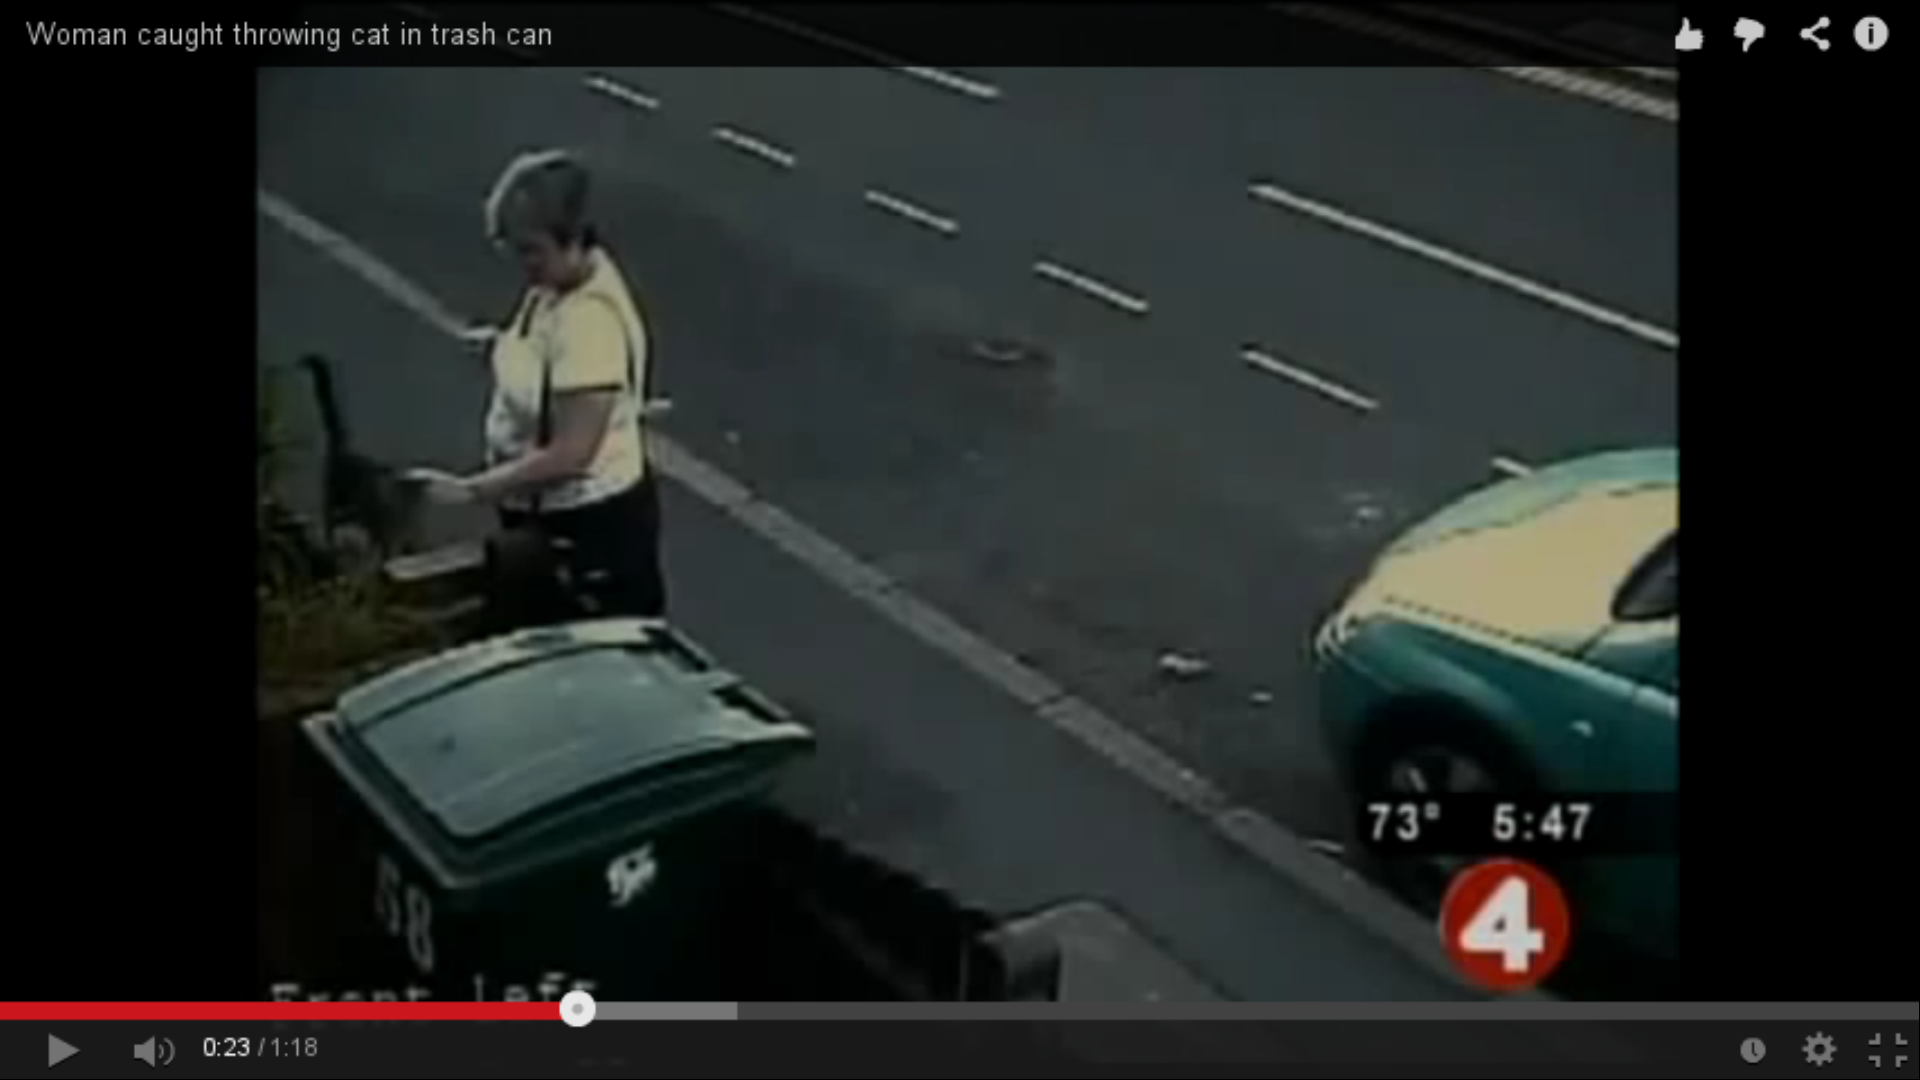
\includegraphics[width=\linewidth]{images/stroke2}\\
            \begin{visibleenv}<2->
            \tiny Stroke cat.
            \end{visibleenv}

            \column{.2\linewidth}
            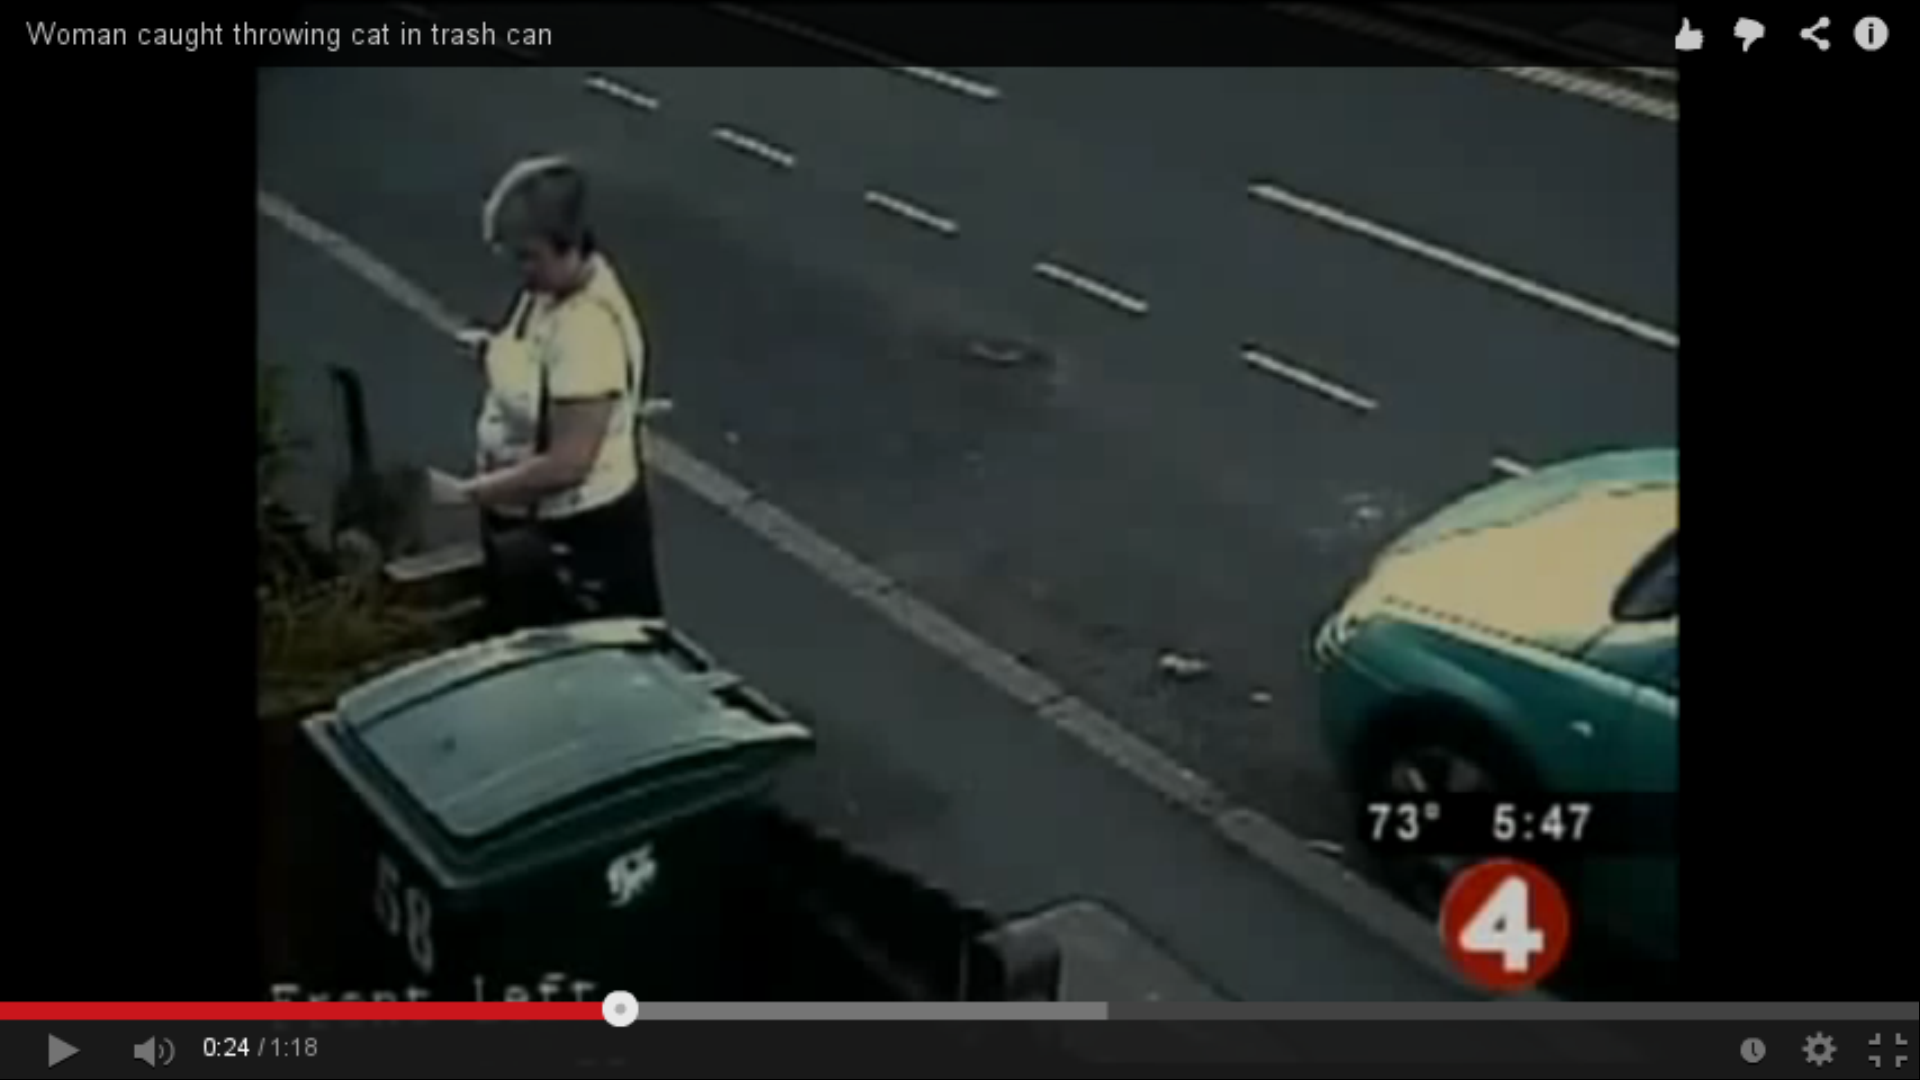
\includegraphics[width=\linewidth]{images/stroke3}\\
            \begin{visibleenv}<2->
            \tiny Stroke cat.
            \end{visibleenv}

            \column{.2\linewidth}
            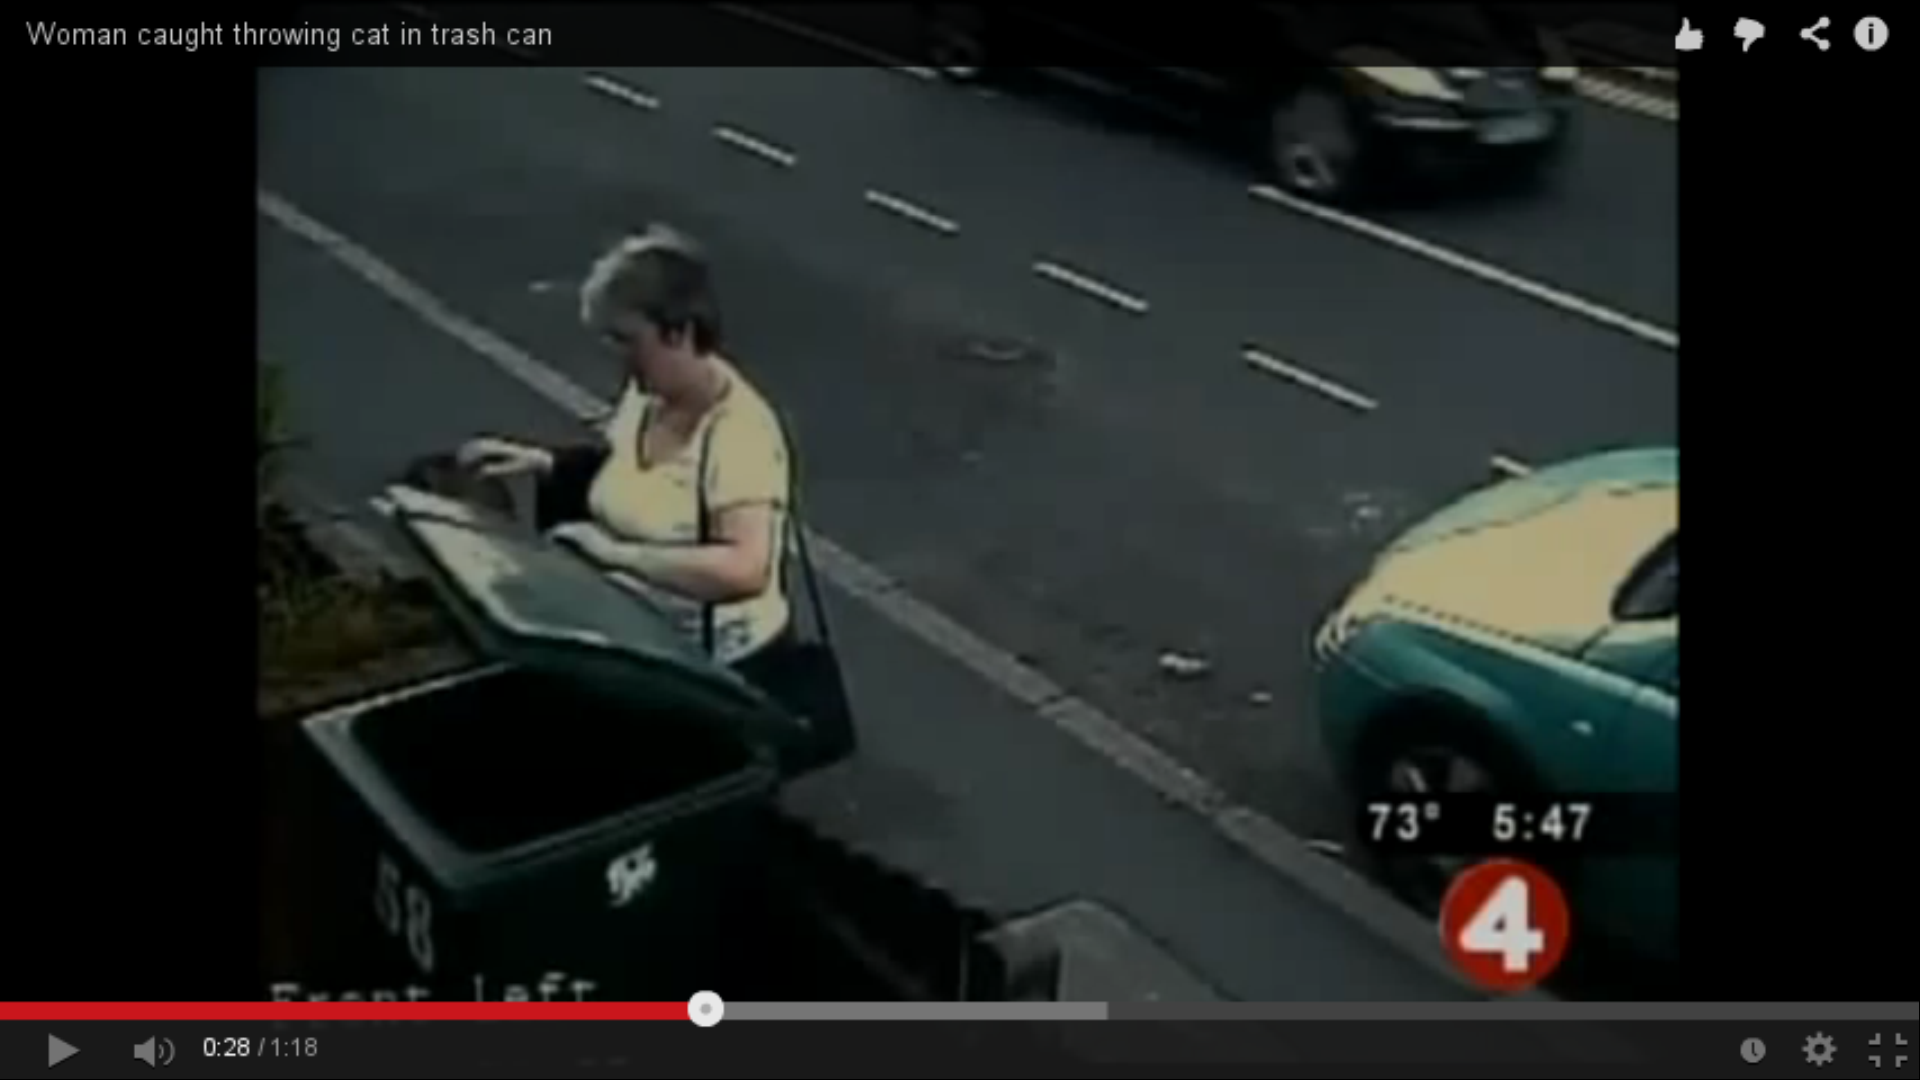
\includegraphics[width=\linewidth]{images/open_trash_can}\\
            \begin{visibleenv}<2->
                \tiny{Open trash can.}
            \end{visibleenv}

            \column{.2\linewidth}
            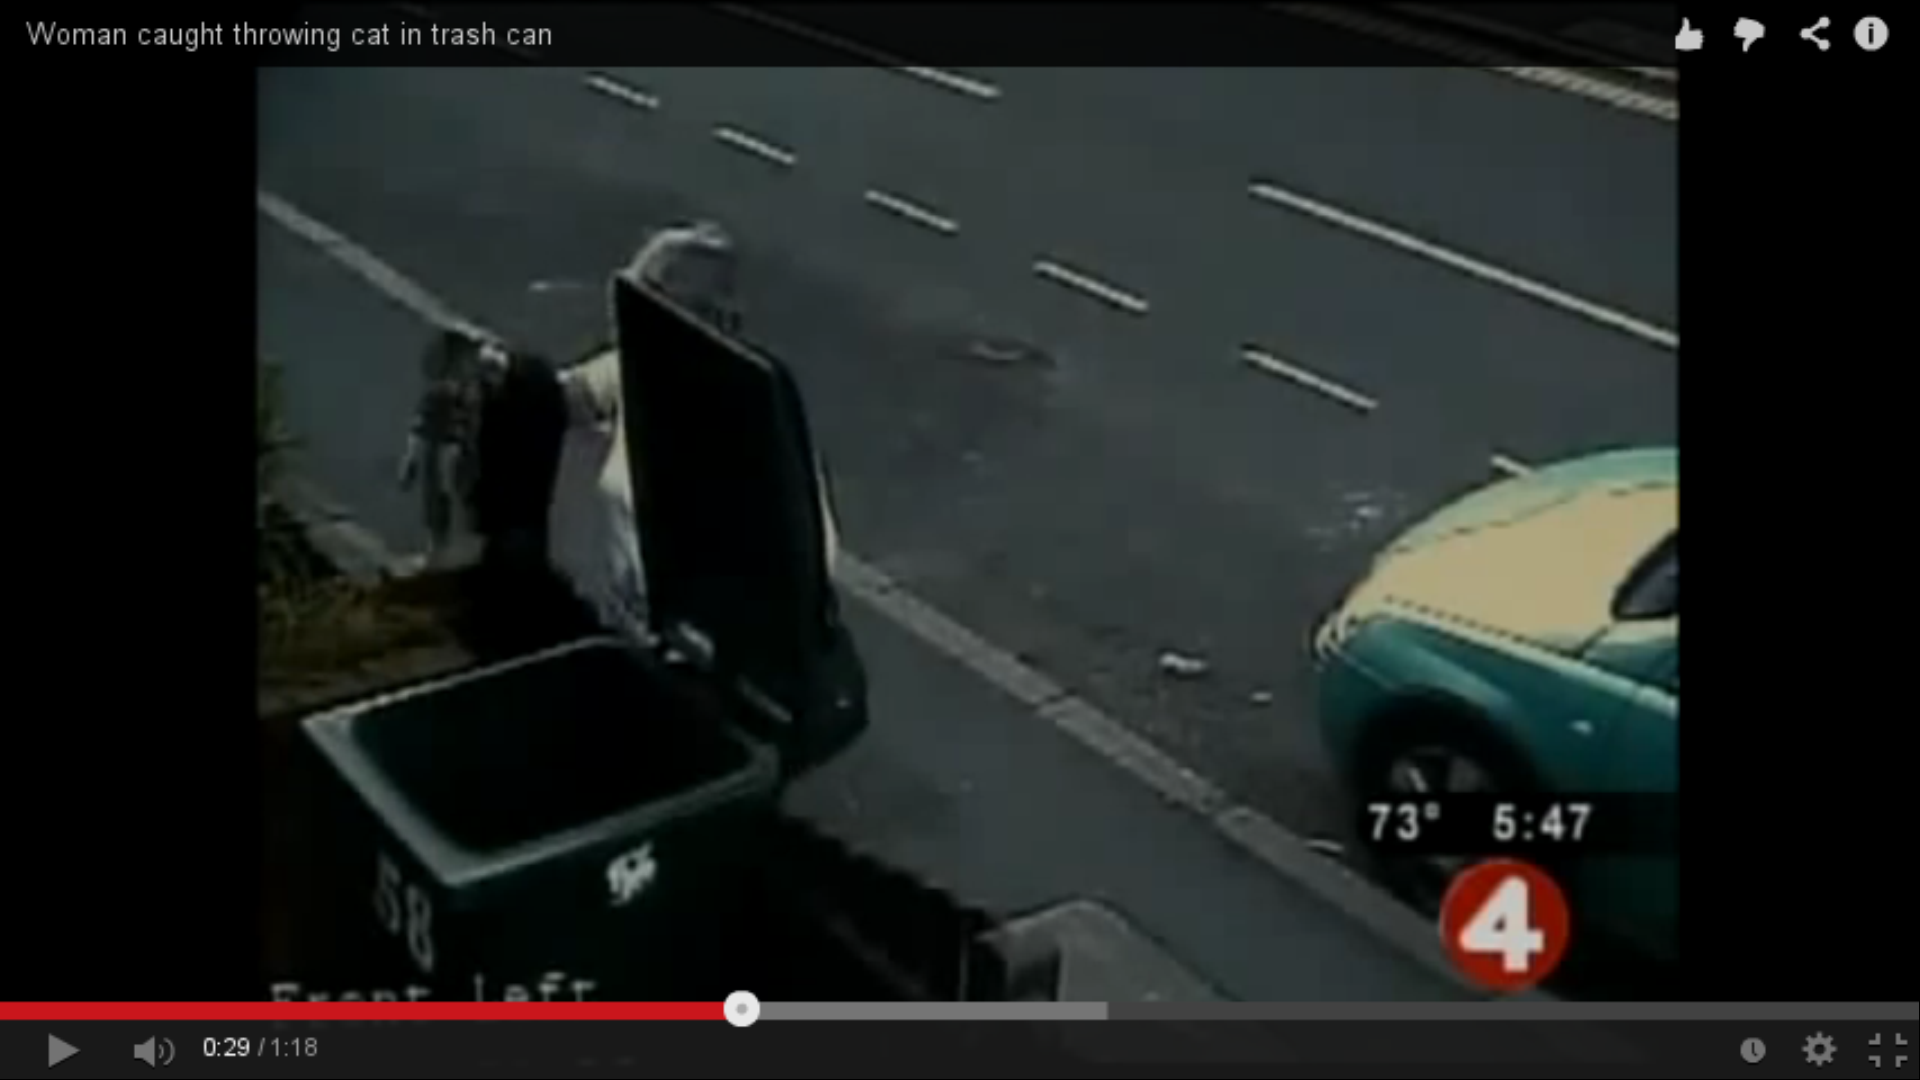
\includegraphics[width=\linewidth]{images/cat_in_trashcan}\\
            \begin{visibleenv}<2->
                \tiny{Put cat in trash can.}
            \end{visibleenv}
        \end{columns}
    \vspace{5mm}
    \begin{center}
    \begin{visibleenv}<3->
            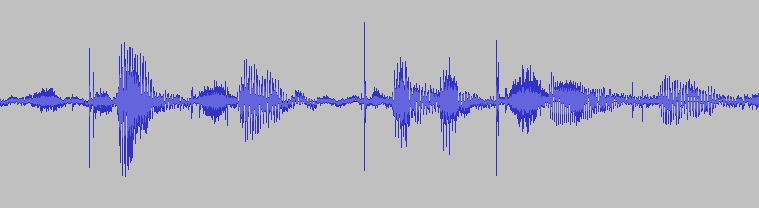
\includegraphics[width=.8\linewidth]{images/speech}\\
    \end{visibleenv}
    \begin{visibleenv}<4->
                Struc-tured pre-dic-tion in Py-thon
    \end{visibleenv}
    \end{center}
    \end{frame}

    \begin{frame}
        \frametitle{Predicting Parse Trees}
        \begin{center}
            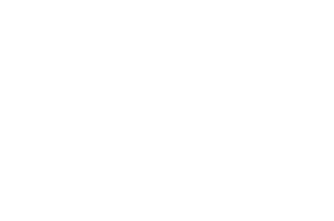
\includegraphics[width=.8\linewidth]{images/parse_tree}
        \end{center}
    \end{frame}

    \begin{frame}
        \frametitle{Semantic Images Segmentation}
        \begin{figure}
            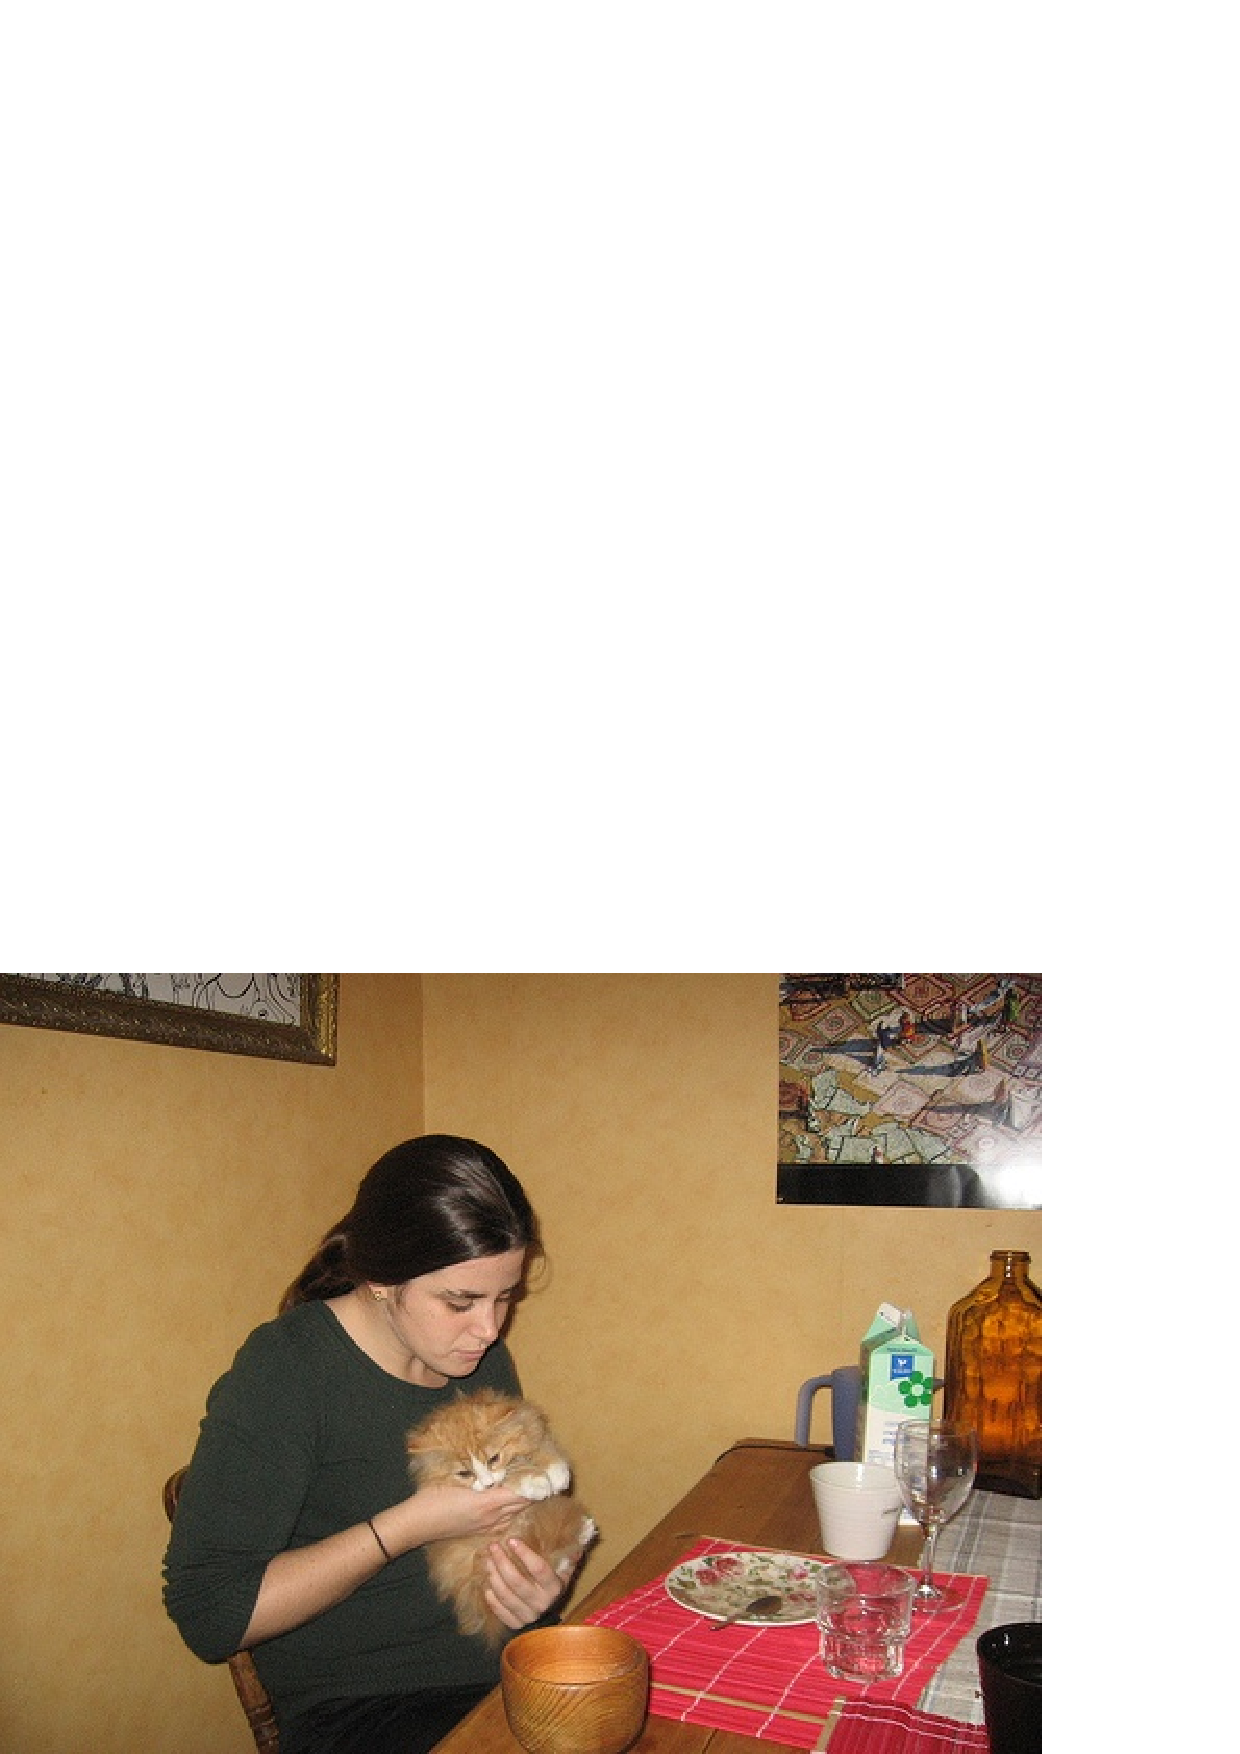
\includegraphics[width=.45 \textwidth]{images/pascal}
            \begin{visibleenv}<2->
                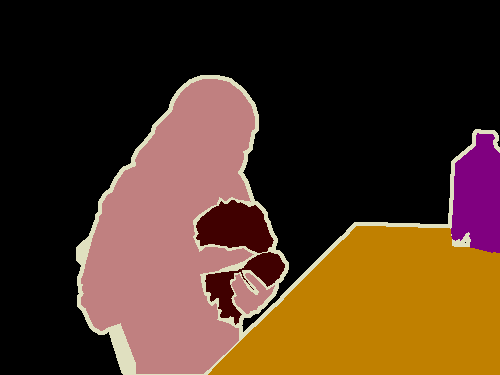
\includegraphics[width=.45 \textwidth]{images/pascal_gt}
            \end{visibleenv}
        \end{figure}
    \end{frame}

    \begin{frame}
        \frametitle{Predicting Structured Objects}
        \[f(x, w) := \argmax_{y \in \mathcal{Y}}  g(x, y, w) \]
        \begin{visibleenv}<2->
        If you like:
        \[\argmax_{y \in \mathcal{Y}}  p(y|x, w) \]
        \end{visibleenv}
        
        \begin{visibleenv}<3>
        \[f(x, w) := \argmax_{y \in \mathcal{Y}}  w^T \psi(x, y) \]
        \end{visibleenv}
    \end{frame}

    \section{Inference and Factor Graphs}
    \begin{frame}
        \frametitle{Predicting discrete vectors}
        \[y = (y_1, y_2, \dotsc, y_{n_i})\]
        \begin{visibleenv}<2>
            \begin{align*}
            f(x, w) &= \argmax_{y \in \mathcal{Y}}  w^T \psi(x, y)\\
                &= \argmax_{y_1, y_2, \dotsc, y_{n_i}} w^T \psi(x, y)
            \end{align*}
        \end{visibleenv}
    \end{frame}

    \begin{frame}
        \frametitle{Factor Graphs}
        \begin{columns}[c]
            \column{.6\linewidth}
            \begin{align*}
            g(x, y) &= g_1(x, y_1, y_2, y_3) + g_2(x, y_3, y_4)\\
                    &+ g_3(x, y_4) + g_4(x, y_4, y_5, y_6)
            \end{align*}
            \column{.3\linewidth}
                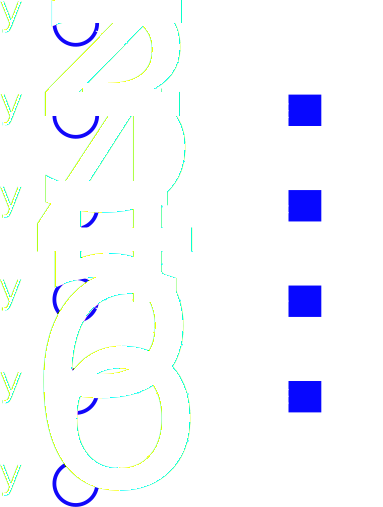
\includegraphics[width=\textwidth]{images/factor_graph}
        \end{columns}
    \end{frame}

    \begin{frame}
        \frametitle{Factor Graph for HMM}
        \begin{center}
            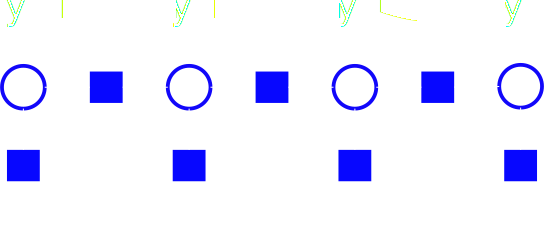
\includegraphics[width=.8\textwidth]{images/hmm}
        \end{center}
    \end{frame}

    \begin{frame}
        \frametitle{Inference}
        \begin{columns}[t]
            \column{.5\linewidth}
            Easy\\
            \vspace{5mm}
            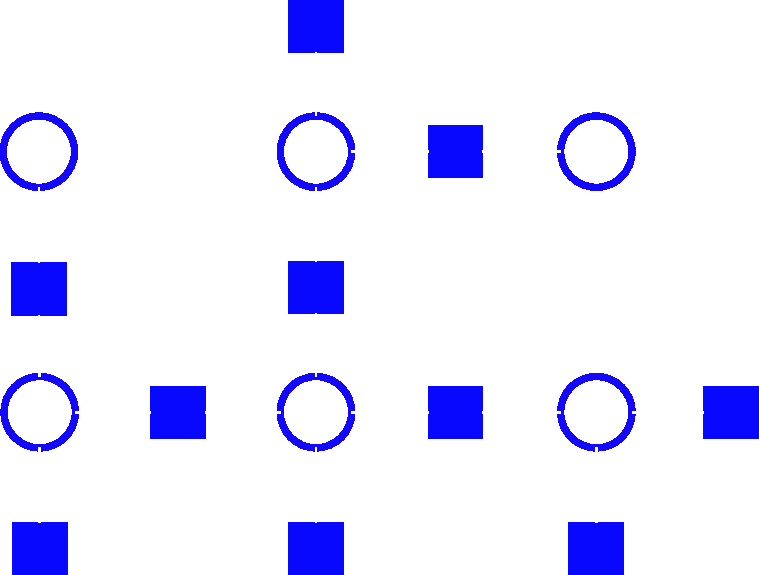
\includegraphics[width=.8\textwidth]{images/tree}
            \column{.5\linewidth}
            Tricky\\
            \vspace{5mm}
            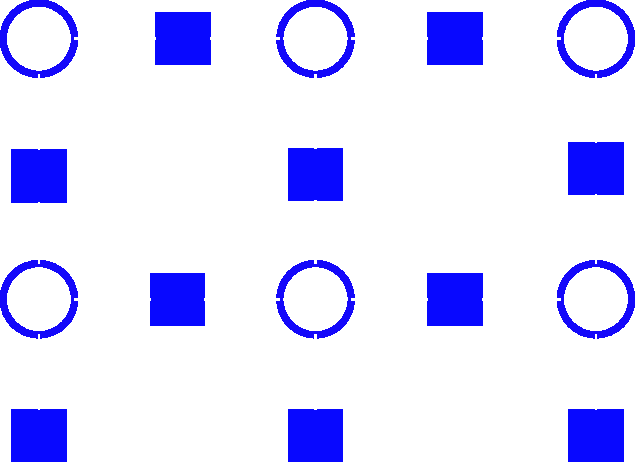
\includegraphics[width=.8\textwidth]{images/grid}
        \end{columns}
    \end{frame}

    \section{Learning}
    \begin{frame}
        \frametitle{Probabilistic Learning}
        \[ p(y|x, w) = \frac{1}{Z} exp(w^T \psi(x, y))\]
        \[Z = \sum_{y' \in \mathcal{Y}} exp(w^T \psi(x, y')) \]
        \begin{visibleenv}<2->
        Objective
        \begin{align*}
            \max_w \sum_i \log(p(y\hoch{i} | x\hoch{i}, w))\\
            = \max_w \sum_i w^T \psi(x\hoch{i}, y\hoch{i}) - \log(Z)
        \end{align*}
        \end{visibleenv}

    \end{frame}

    \begin{frame}
        \frametitle{Max-Margin Learning}
        \begin{align*}
            &\min_w \frac{1}{2} ||w||^2 + C \sum_i  \ell(x\hoch{i}, y\hoch{i}, w)\\
            &\ell(x\hoch{i}, y\hoch{i}, w) = [\max_{y \in \mathcal{Y}} \Delta(y\hoch{i}, y) + w^T \psi(x\hoch{i}, y) - w^T \psi(x\hoch{i}, y\hoch{i})]_+.
        \end{align*}
    \end{frame}


    \section{PyStruct}
    \begin{frame}
        \frametitle{Simple structured prediction}
        Estimator = Learner + Model + Inference\\

        \begin{itemize}
            \item<2-> Learner: SubgradientSSVM, StructuredPerceptron, OneSlackSSVM, LatentSSVM
            \item<2-> Model: BinaryClf, MultiLabelClf, ChainCRF, GraphCRF, EdgeFeatureGraphCRF
            \item<2-> Inference: Linear Programming, QPBO (PyQPBO), Dual Decomposition (AD3), Message Passing (OpenGM), Everything (OpenGM)
        \end{itemize}

    \end{frame}

    \begin{frame}
        \frametitle{Example OCR}
        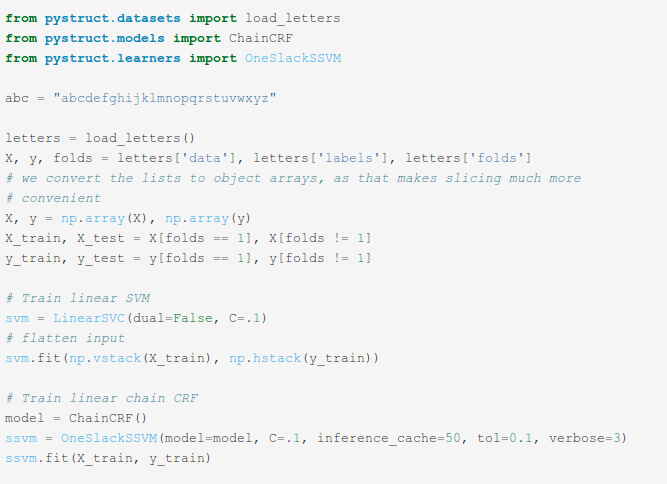
\includegraphics[width=.7\linewidth]{images/code_letters}
    \end{frame}

    \begin{frame}
        \frametitle{Example OCR}
        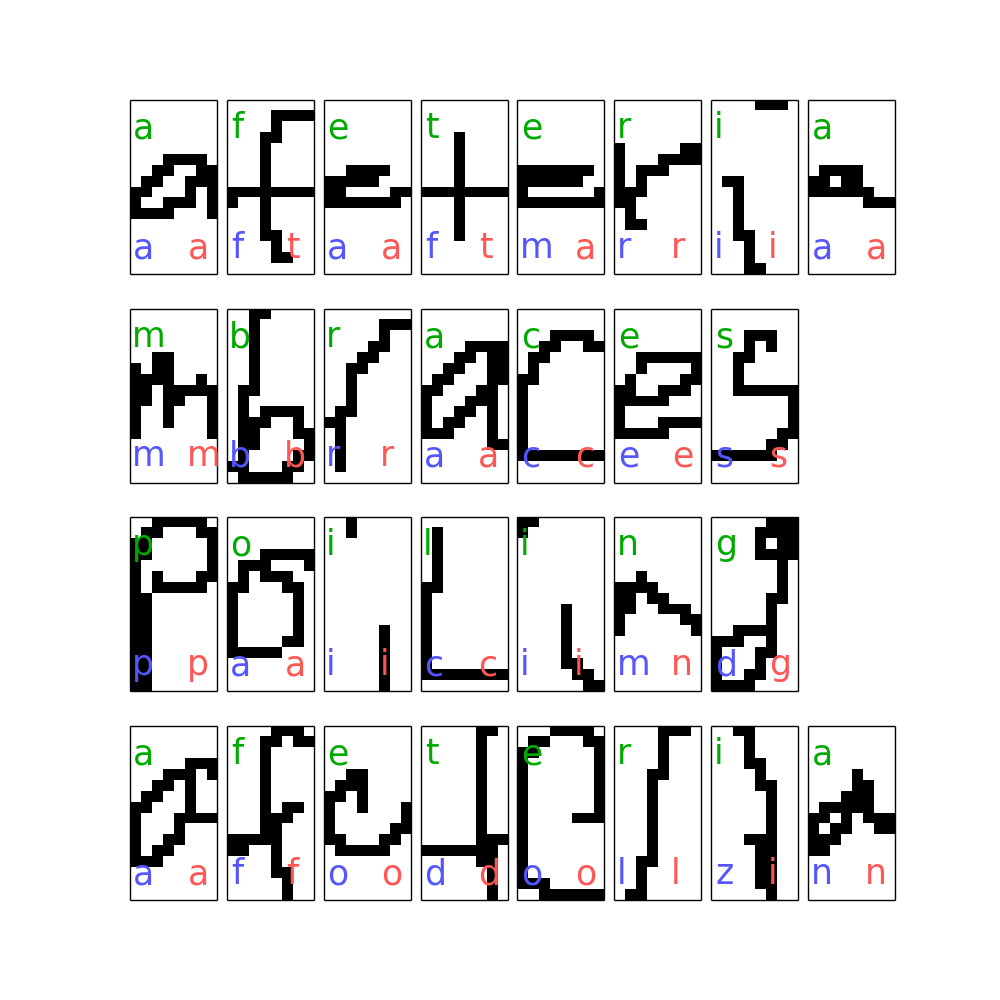
\includegraphics[width=.49\linewidth]{images/plot_letters_1}
        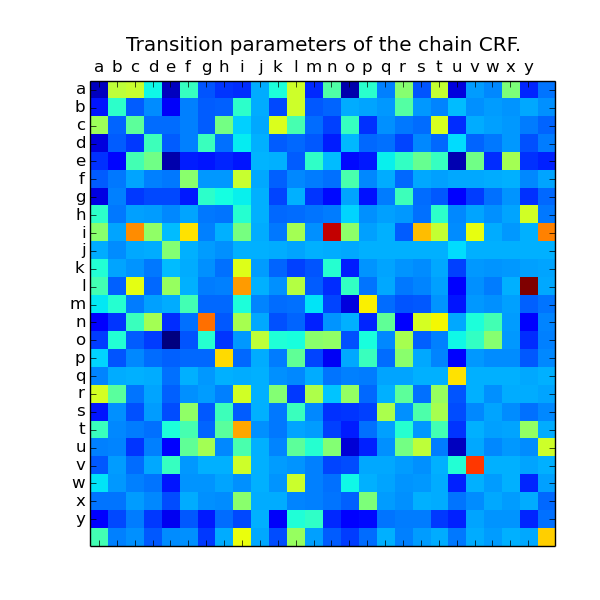
\includegraphics[width=.49\linewidth]{images/plot_letters_2}
    \end{frame}

    \begin{frame}
        \frametitle{Example Snake}
        \begin{center}
            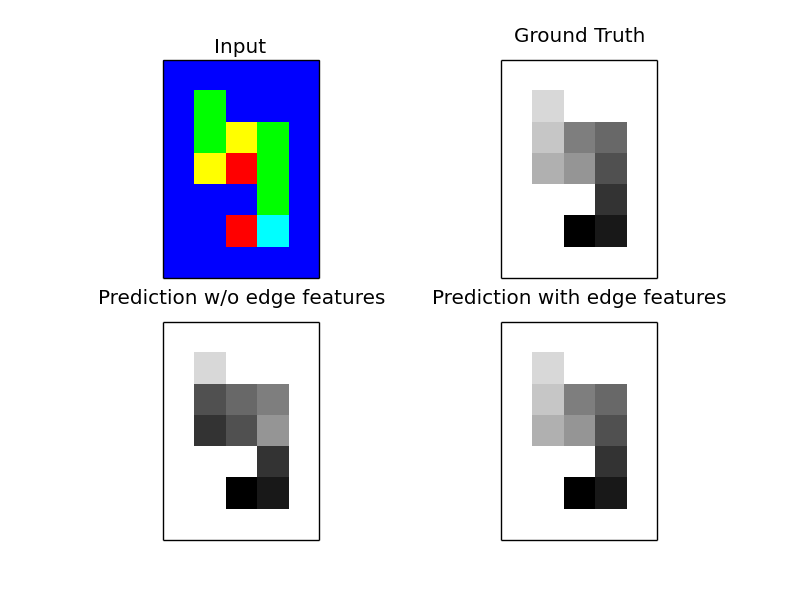
\includegraphics[width=.70\linewidth]{images/plot_snakes_1}
        \end{center}
    \end{frame}

    \begin{frame}
        \begin{center}
            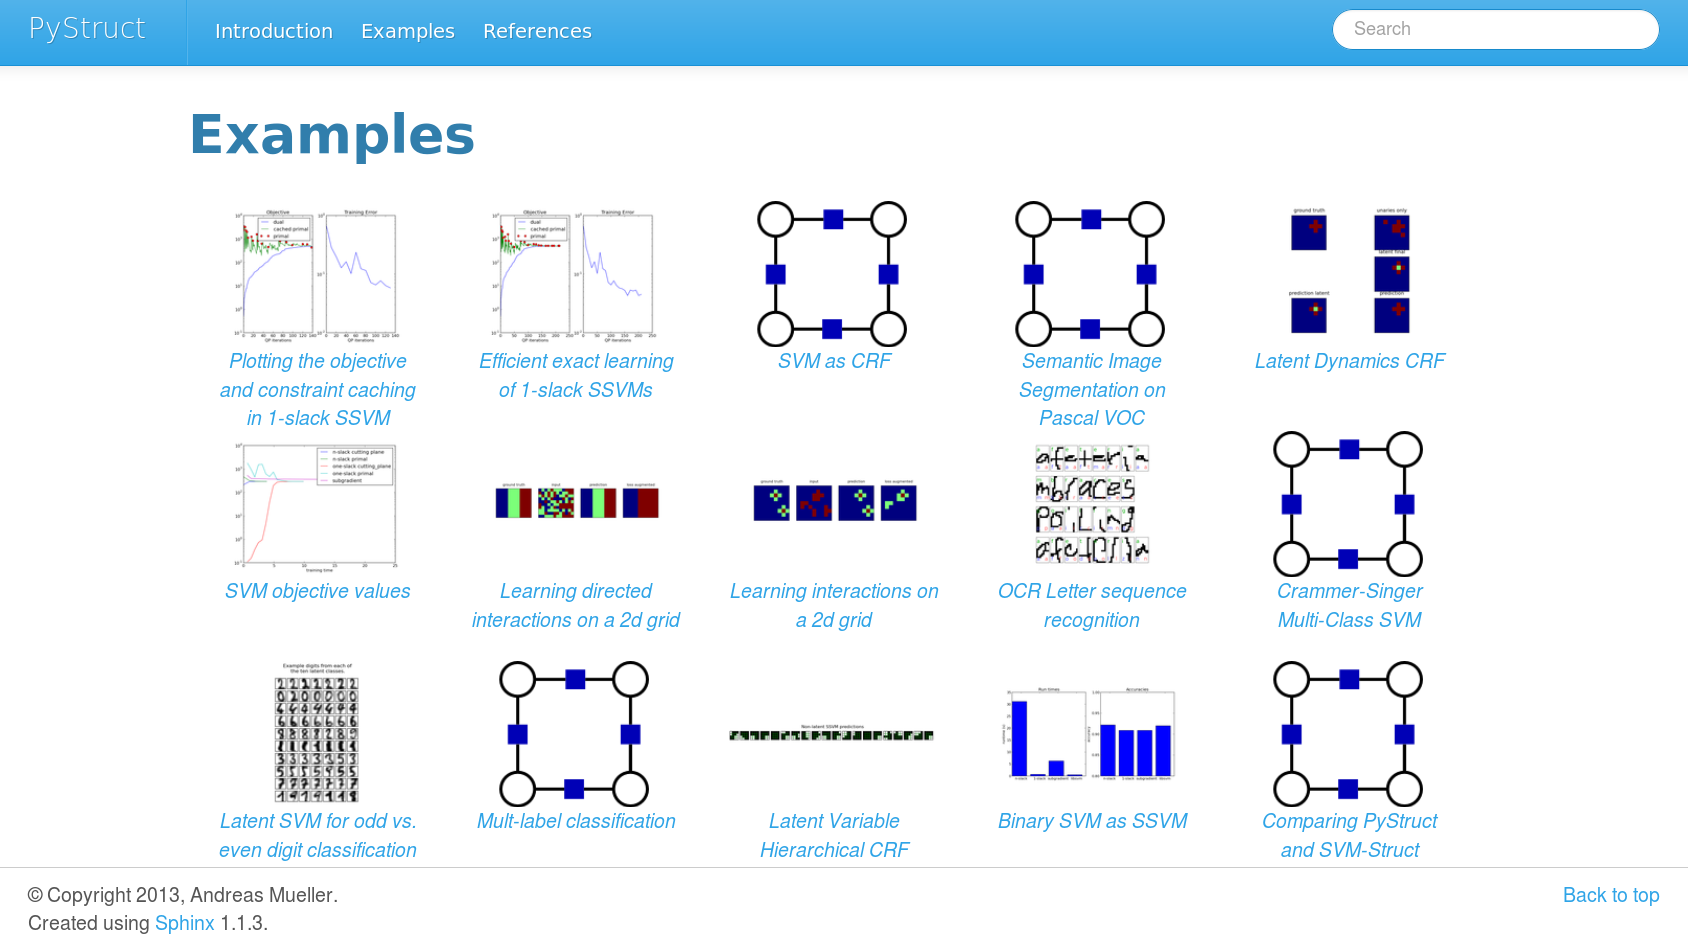
\includegraphics[width=\linewidth]{images/example_gallery}\\
            http://pystruct.github.io
        \end{center}
    \end{frame}
    
	\end{document}
